% Connes invariant S(M) for each factor type, drawn on the half-line R_{>=0}.
% Linear scale; the III_lambda ladder uses lambda = 1/2 and is computed as
% lambda^n for n = -2..12 (points below ~1e-3 merge into the accumulation at 0).
% Included at 0.95\textwidth (6.18in); drawn at ~1:1.
\documentclass[tikz,border=4pt]{standalone}
\usepackage[T1]{fontenc}
\usepackage{lmodern}
\usepackage{amsmath,amssymb}
\usepackage{xcolor}
\usetikzlibrary{arrows.meta}

\definecolor{ruleblue}{HTML}{2b6cb0}
\definecolor{rulegold}{HTML}{b7791f}
\definecolor{rulered}{HTML}{c0392b}
\definecolor{rulegreen}{HTML}{1f8a5f}
\definecolor{axisgray}{HTML}{8a8f98}

\begin{document}
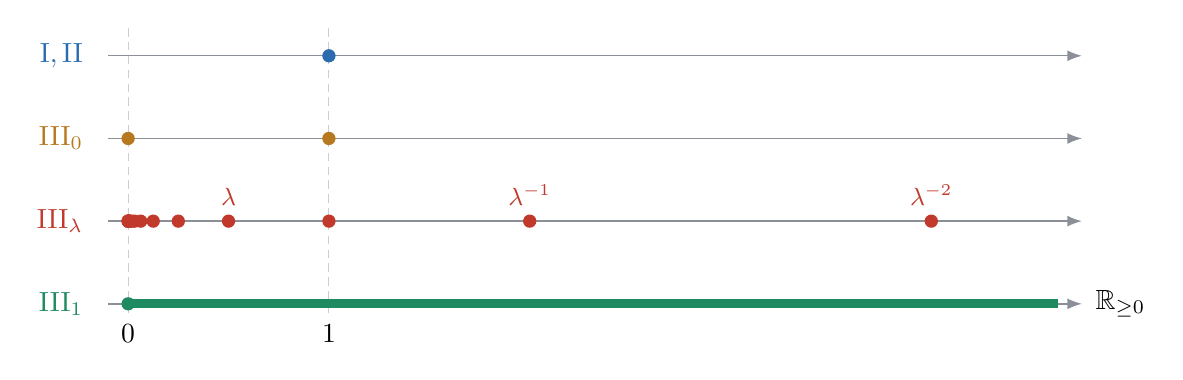
\begin{tikzpicture}[>=Latex, font=\normalsize]
  \def\u{2.55}      % cm per unit of the spectrum axis
  \def\xmax{4.75}   % axis runs 0 .. xmax
  \def\dy{1.05}     % row spacing
  \def\r{2.4pt}     % dot radius

  % faint guides at 0 and 1 across all rows
  \foreach \v in {0,1}
    \draw[axisgray!45, densely dashed, line width=0.4pt]
      ({\v*\u}, 0.35) -- ({\v*\u}, {-3*\dy-0.18});

  % row axes
  \foreach \k in {0,1,2,3}
    \draw[->, axisgray, line width=0.5pt] (-0.25, {-\k*\dy}) -- ({\xmax*\u}, {-\k*\dy});

  % row labels
  \node[anchor=east, ruleblue]  at (-0.45, 0)        {I,\,II};
  \node[anchor=east, rulegold]  at (-0.45, -\dy)     {III$_0$};
  \node[anchor=east, rulered]   at (-0.45, {-2*\dy}) {III$_\lambda$};
  \node[anchor=east, rulegreen] at (-0.45, {-3*\dy}) {III$_1$};

  % Types I and II: {1}
  \fill[ruleblue] (\u, 0) circle (\r);

  % Type III_0: {0, 1}
  \fill[rulegold] (0, -\dy) circle (\r);
  \fill[rulegold] (\u, -\dy) circle (\r);

  % Type III_lambda: {0} u lambda^Z, lambda = 1/2
  \begin{scope}[shift={(0,{-2*\dy})}]
    \foreach \n in {-2,...,12} {
      \pgfmathsetmacro{\v}{0.5^\n}
      \fill[rulered] ({\v*\u}, 0) circle (\r);
    }
    \fill[rulered] (0, 0) circle (\r);
    \node[rulered, above=2pt, font=\small] at ({0.5*\u}, 0) {$\lambda$};
    \node[rulered, above=2pt, font=\small] at ({2*\u}, 0) {$\lambda^{-1}$};
    \node[rulered, above=2pt, font=\small] at ({4*\u}, 0) {$\lambda^{-2}$};
  \end{scope}

  % Type III_1: the whole half-line
  \draw[rulegreen, line width=3.2pt] (0, {-3*\dy}) -- ({(\xmax-0.12)*\u}, {-3*\dy});
  \fill[rulegreen] (0, {-3*\dy}) circle (\r);

  % shared tick labels
  \node[below=4pt] at (0, {-3*\dy}) {$0$};
  \node[below=4pt] at (\u, {-3*\dy}) {$1$};
  \node[anchor=west] at ({\xmax*\u+0.05}, {-3*\dy}) {$\mathbb{R}_{\ge 0}$};
\end{tikzpicture}
\end{document}
